\begin{frame}{Numerics}

    \begin{minipage}{.49\textwidth}
        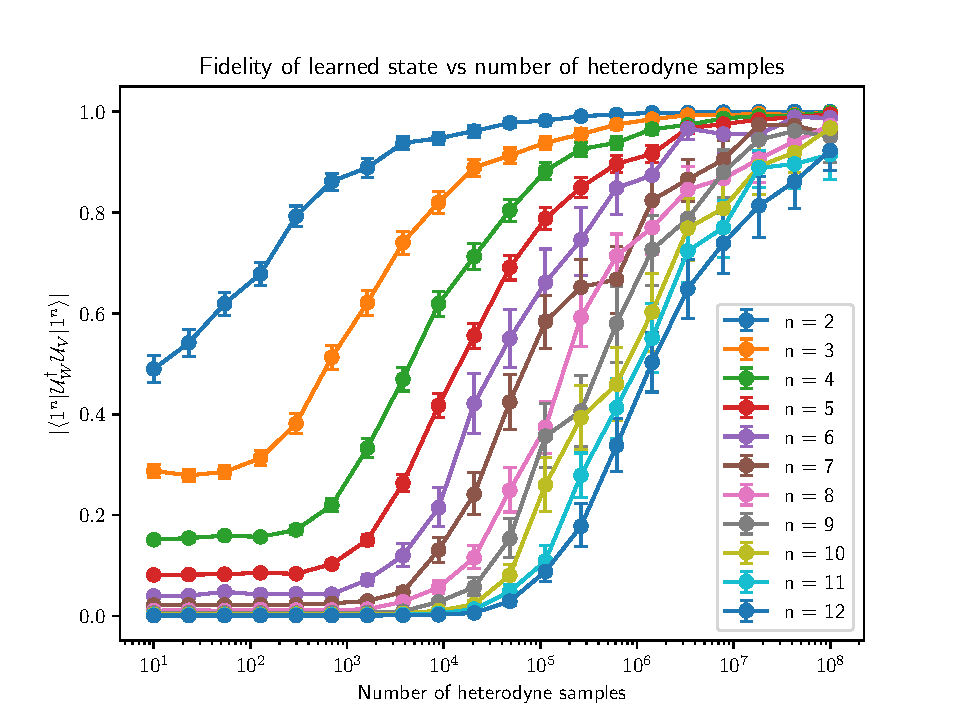
\includegraphics[width=1.1\textwidth]{graphics/sample.pdf}
    \end{minipage}
    \hfill
    \begin{minipage}{.49\textwidth}
        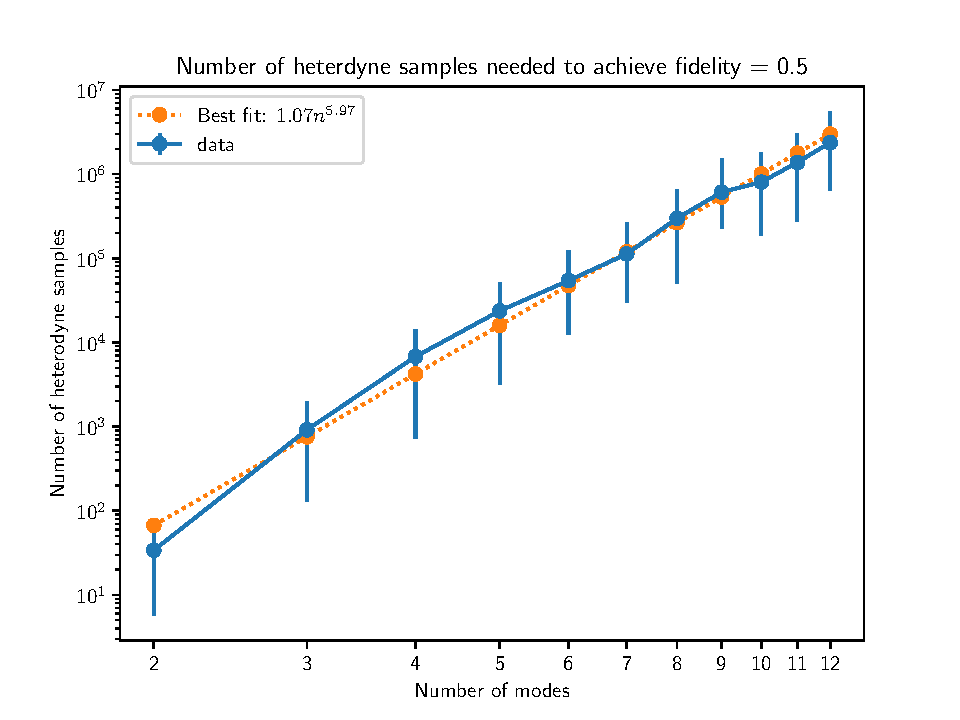
\includegraphics[width=1.1\textwidth]{graphics/threshold.pdf}
    \end{minipage}

\end{frame}


\begin{frame}{Sketch of our algorithm}
    \begin{spaceditemize}
        \item For simplicity, we will restrict our attention here to \\[1em]
        ~~~~~passive Gaussian unitaries (specified by \(W \in \U(n)\))\\[1em]
        ~~~~~the Fock state \(\ket{1,\dots,1} \equiv \ket{1^n}\)\\[1em]
        ~~~~~the error free case (assume moments are known \emph{perfectly})\\[1em]
        \item We sketch the learning algorithm for \(\calU_W\ket{1^n}\) with these simplicifcations
    \end{spaceditemize}

\end{frame}

\begin{frame}{Passive moment transformations}
    \begin{spaceditemize}
        \item Recall \( W\in U(n) \) acts as
        \[\calU_W^\dag a_i \calU_W = \sum_{j} W_{ij} a_j \]
        \item How do moments \textbf{transform}?
        \begin{align*}
             & \sigma^{(t)}_{i_1,\dots,i_t; j_1,\dots,j_t} = \bra{1^n}\calU_W^\dag a_{i_1}\dots a_{i_t}a^\dag_{j_1}\dots a^\dag_{j_t} \calU_W\ket{1^n} \\
            %
             & (\sigma^{(t)}_0)_{i_1,\dots,i_t; j_1,\dots,j_t} = \bra{1^n} a_{i_1}\dots a_{i_t}a^\dag_{j_1}\dots a^\dag_{j_t}\ket{1^n}                 \\
            %
             & \sigma^{(t)} = W^{\otimes t}\sigma^{(t)}_0 W^{\dag \otimes t}
        \end{align*}
        %
        \item \(\sigma^{(t)}\) is a submatrix of a unitary transformation of the \(\Lambda^{(t)}\) moments
    \end{spaceditemize}

\end{frame}


\begin{frame}{Reducing the problem}
    \begin{spaceditemize}
        \item If we were dealing with Gaussian states, \(\sigma^{(1)}\) would be sufficient
        \item But for us \textbf{second moments are useless} --- easy to check that \(\sigma^{(1)}_0 \propto \bbI\)
        \item Therefore, \(\sigma^{(1)} = W \sigma^{(1)}_0 W^\dag = \sigma^{(1)}_0\), so we learn nothing about \(W\) by measuring second moments
        \item So now we use \textbf{fourth moments}, \(\sigma^{(2)}\)
    \end{spaceditemize}
\end{frame}


\begin{frame}{Learning algorithm}
    \begin{block}{}
        Given the fourth moments \(\sigma^{(2)} = W^{\otimes 2} \sigma^{(2)}_0 W^{\dag \otimes 2}\) for the state \(\calU_W \ket{1^n}\), determine \(W\)
    \end{block}
    \vfill
    \begin{spaceditemize}[0em]
        % \item Recall we are still assuming that $\sigma^{(4)}$ is known perfectly
        \item Because \( \sigma^{(2)}_0 \) is a matrix on \( (\bbC^{n})^{\otimes 2} \), we can represent it in bra-ket notation using the standard basis \( \ket{1},\dots,\ket{n} \) of \( \bbC^n \)
        % .
        % Easy to check that 
        \begin{equation*}
            \sigma^{(2)}_0 = 4 (\bbI + U_{\rm SWAP})
            - 2\sum_{i=1}^{n}\ket{i,i}\bra{i,i},
        \end{equation*}
        \item Denote the \( i^{\rm th} \) column vector of \( W \) by \( \ket{w_i} \).
        Given access to \(\sigma^{(2)}\), we can thus form the matrix
        \begin{align*}
            A & = \frac{1}{2}\parentheses{4(\mathbb I + U_{\rm SWAP}) - \sigma^{(2)}}     \\
            %
              & =  \sum_{i=1}^n (\ket{w_i}\otimes \ket{w_i})(\bra{w_i}\otimes \bra{w_i}),
        \end{align*}
    \end{spaceditemize}
\end{frame}

\begin{frame}{Learning algorithm}
    \begin{block}{}
        Given access to a matrix \(A = \sum_{i=1}^n (\ket{w_i}\otimes \ket{w_i})(\bra{w_i}\otimes \bra{w_i})\), learn \(\ket{w_i}\) (up to phases and permutations)
    \end{block}
    \vfill
    \begin{spaceditemize}
        \item Unitarily diagonalize \(A\) and take the \(+1\) eigenvalues --- we learn the eigenspace \(\text{span}\cbargs{\ket{w_i}\otimes \ket{w_i} \mid i=1,\dots, n}\)
        \item A numerical diagonalization routine will return the vectors
        \begin{equation*}
            \ket{\tilde w_i} = \sum_{j=1}^n U_{ij}\ket{w_j}\otimes \ket{w_j}
            =
            \sum_{j=1}^n \abs*{U_{ij}}e^{\i\phi_{ij}}\ket{w_j}\otimes \ket{w_j}
        \end{equation*}
        \item Take the intersection of the Schmidt decompositions of all \(\ket{\tilde w_i}\) to learn all the \(\ket{w_i}\) up to phases
    \end{spaceditemize}
\end{frame}

\begin{frame}{Learning algorithm}

    \begin{spaceditemize}[2em]
        \item We have therefore learned the matrix \(V = W \Phi P\), where \(\Phi\) is some arbitrary diagonal unitary matrix, and \(P\) is some arbitrary permutation matrix
        \item It follows that the state \( \calU_V \ket{1^n} \) is the same as \( \calU_W \ket{1^n} \) up to an irrelevant global phase, thereby completing the learning algorithm
        \item To prove the main result, we need to track how the error in the moments propagates through the algorithm to an error in the fidelity
    \end{spaceditemize}

\end{frame}
